\clearpage
%%%%%%%%%%%%%%%%%%%%%%%%%%%%%%%%%%
\section{Discussion}
\label{sec:discussion}
%%%%%%%%%%%%%%%%%%%%%%%%%%%%%%%%%%

Figure~\ref{fig:inc_cut_kt} compares several differential distribution computed using the two approaches. For the collinear approach pure inelastic contribution is estimated by
subtracting elastic part computed following Eq.~\ref{eq:elasticRenat}.
For the invariant mass distribution and lepton pseudorapidity the shapes are similar and
the main difference between the two predictions is observed in the normalization.
For the distribution of the lepton pair rapidity the two predictions agree at larger rapidities while disagreement concentrates
in the central region. The biggest difference is observed for the transverse momentum distribution of the lepton where at low $p_T$ collinear approximation exceeds the estimate
from $k_T$-factorization approach while at high $p_T$ the ordering is reversed.  
This suggests that at low $p_T$ (close to the boundary of the fiducial region) the difference is due to the smearing of dilepton transverse momentum introduced by the $k_T$-factorization approach.

We also take the opportunity to calculate expected number of events for realistic assumption on total integrated luminosity.
Based on the previous $p+\textrm{Pb}$ runs at the LHC, we assume  $\int Ldt= 200~\textrm{nb}^{-1}$.
We also assume possible experimental efficiencies, mainly due to trigger and reconstruction of leptons, which we embed in a single correction factor $C=0.7$.

Table~\ref{fig:numbers} shows the expected number of events for $p+\textrm{Pb}\rightarrow \textrm{Pb} + \ell^+\ell^- + X$ production at $\sqrt{s_{N N}} = 8.16$~\TeV\ and configuration described above. 
Approximately 2500 elastic dilepton events are expected. 
Depending on the calculations, 3400 (collinear with LUXqed17 PDF) or 2400 ($k_T$-factorization with LUX-like $F_2+F_L$) reconstructed inelastic events are predicted. 
%The difference between collinear and $k_T$-factorization can be therefore constrained with large significance, using existing datasets collected by ATLAS and CMS.
The data should be therefore sensitive to discriminate between the predictions based on  
collinear and $k_T$-factorization approaches, using existing datasets collected by ATLAS and CMS.



\begin{figure}[]
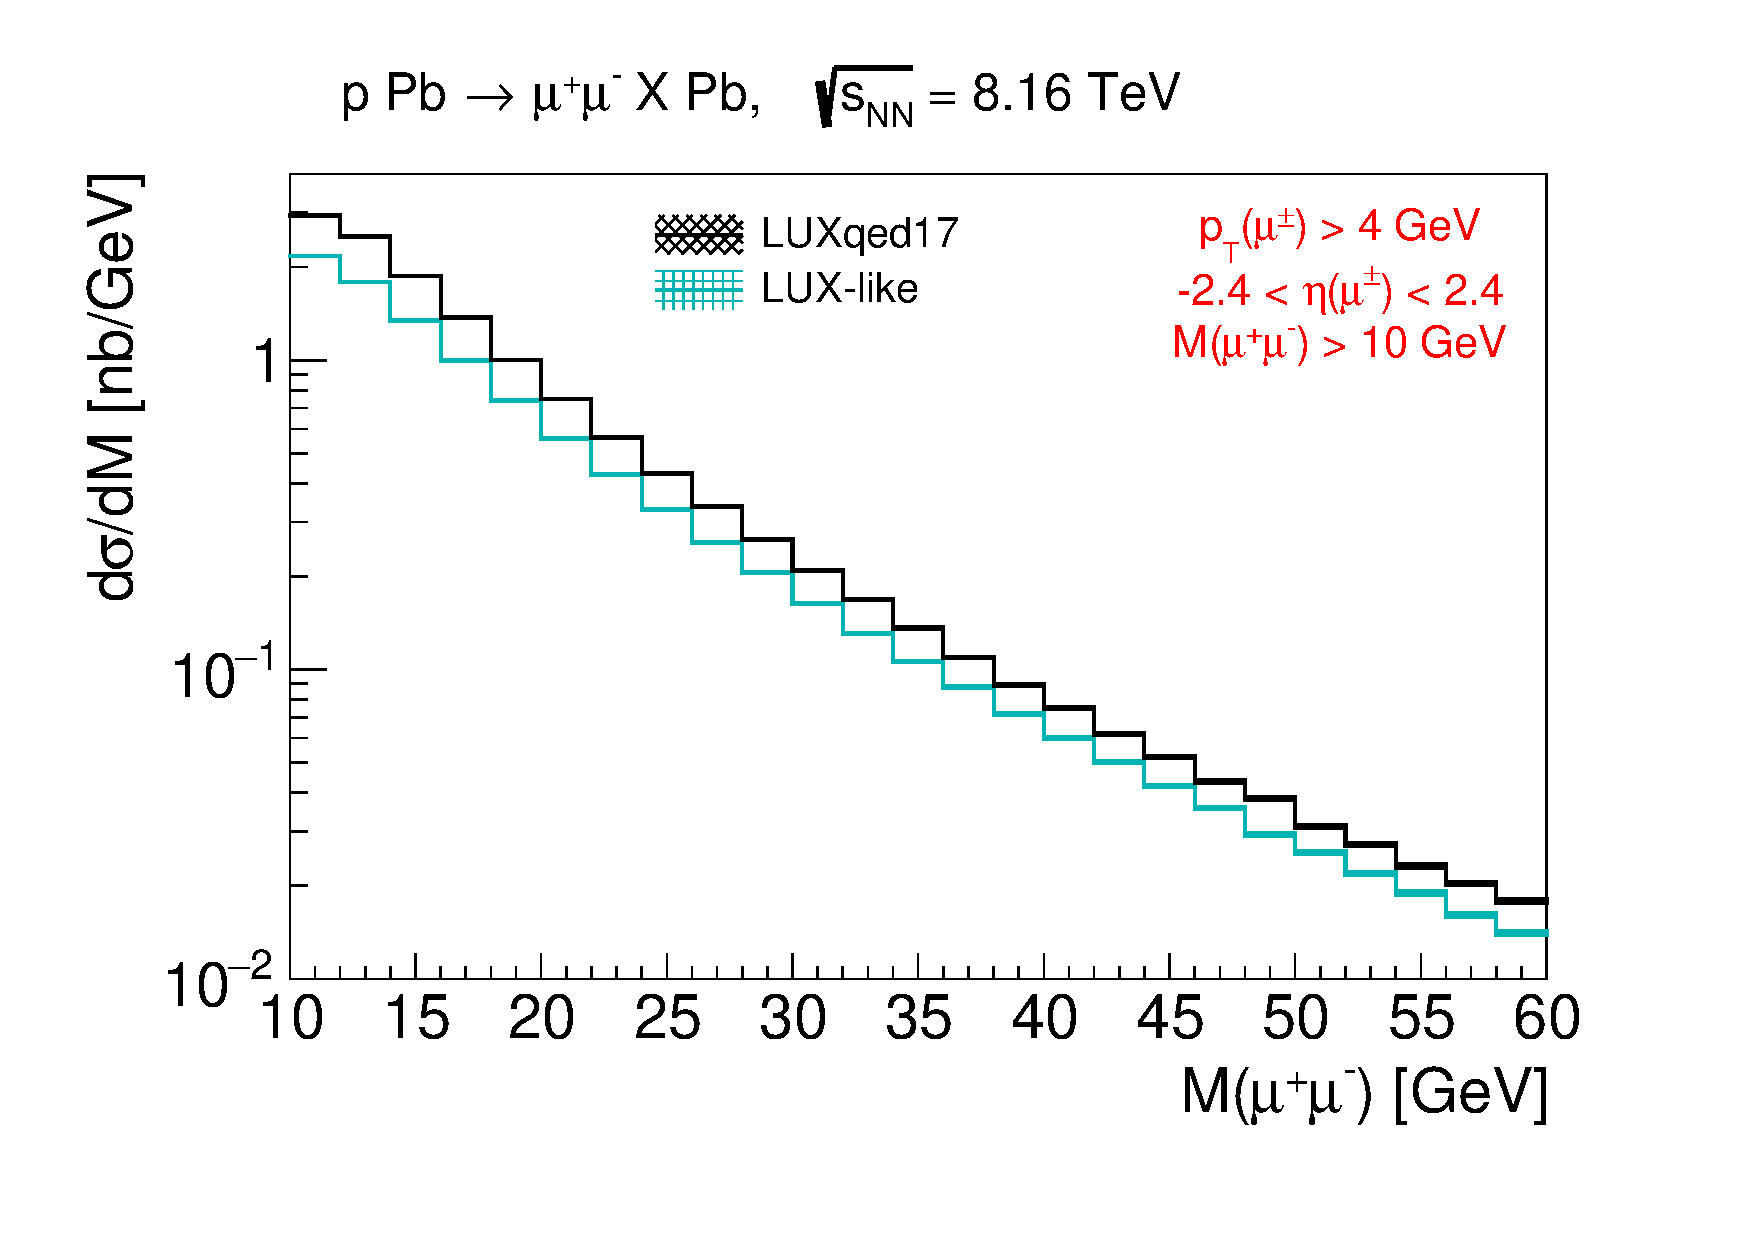
\includegraphics[width=0.43\textwidth]{figures/Mll_inc_cut_kt.pdf}
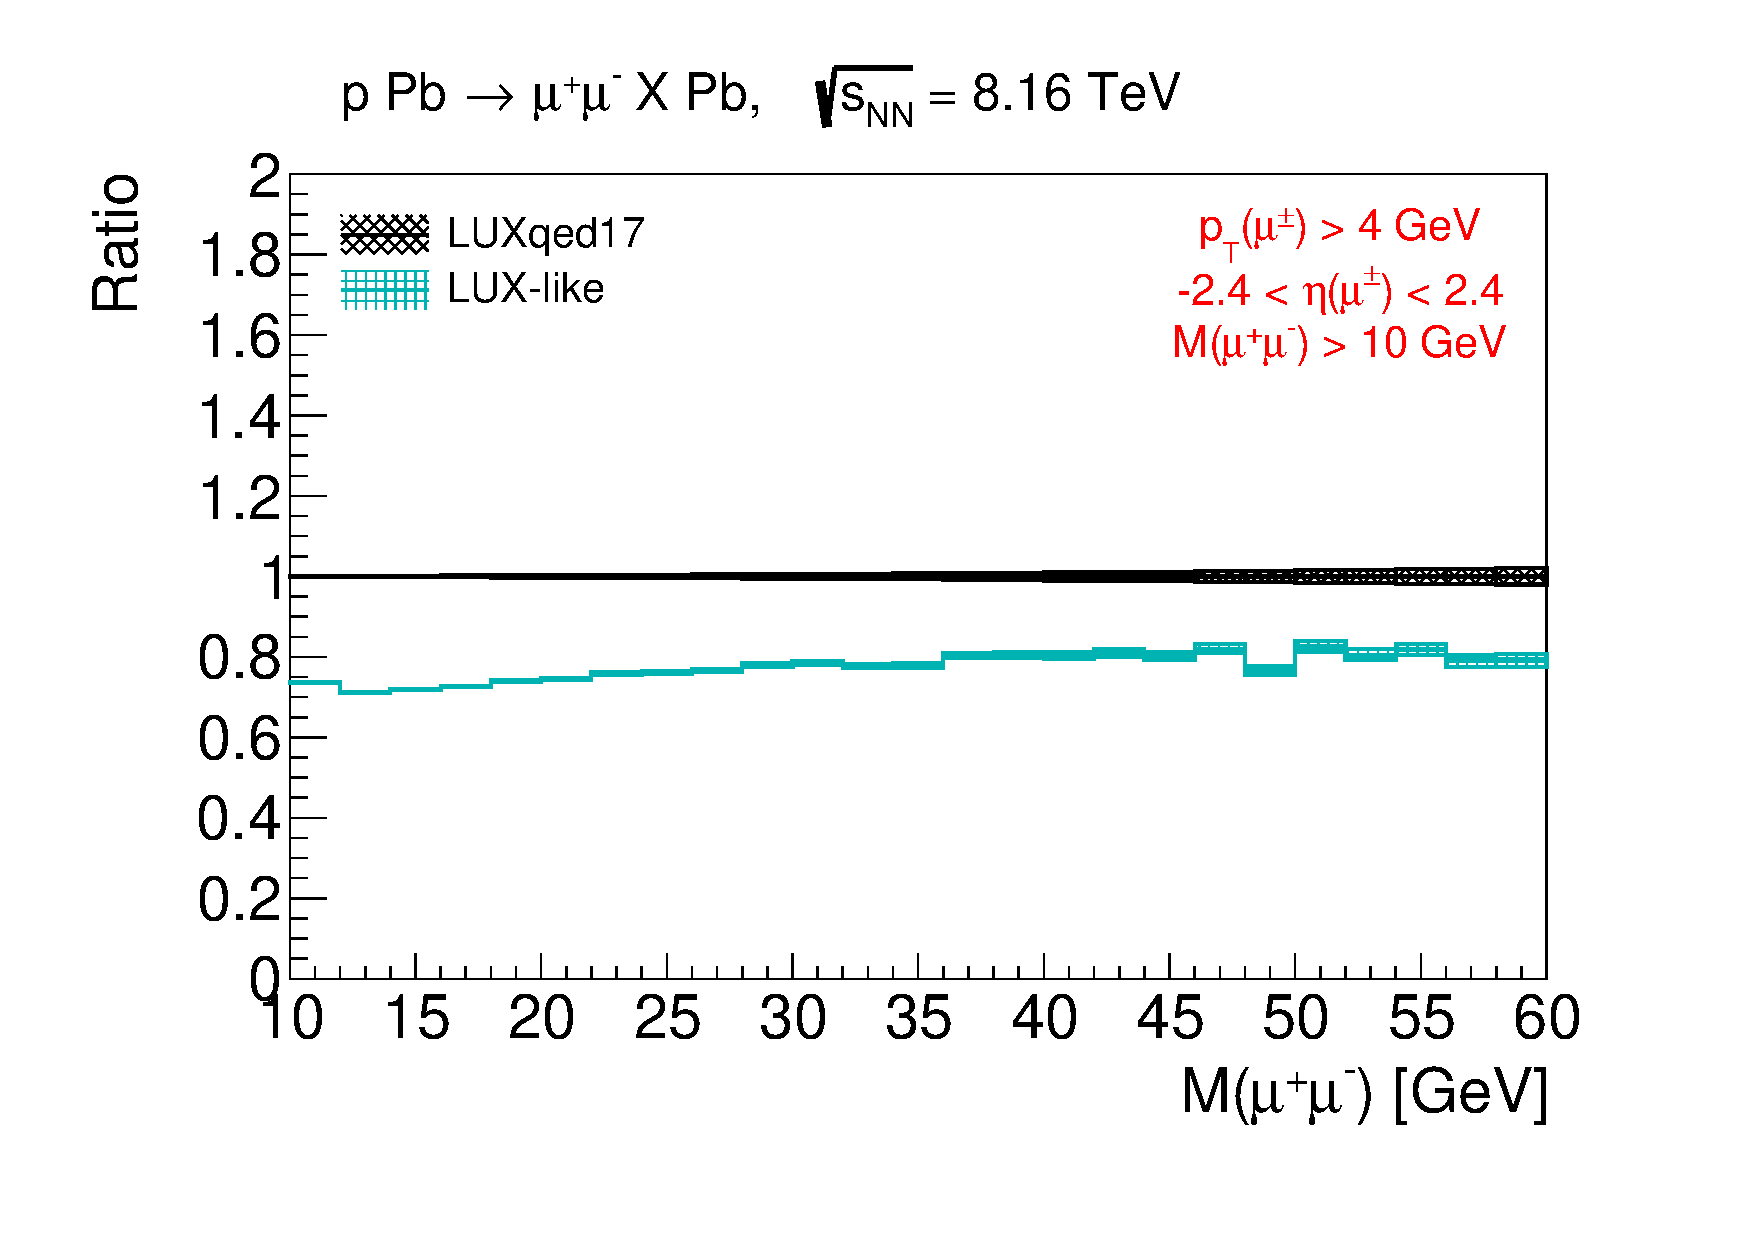
\includegraphics[width=0.43\textwidth]{figures/RatioMll_inc_cut_kt.pdf}
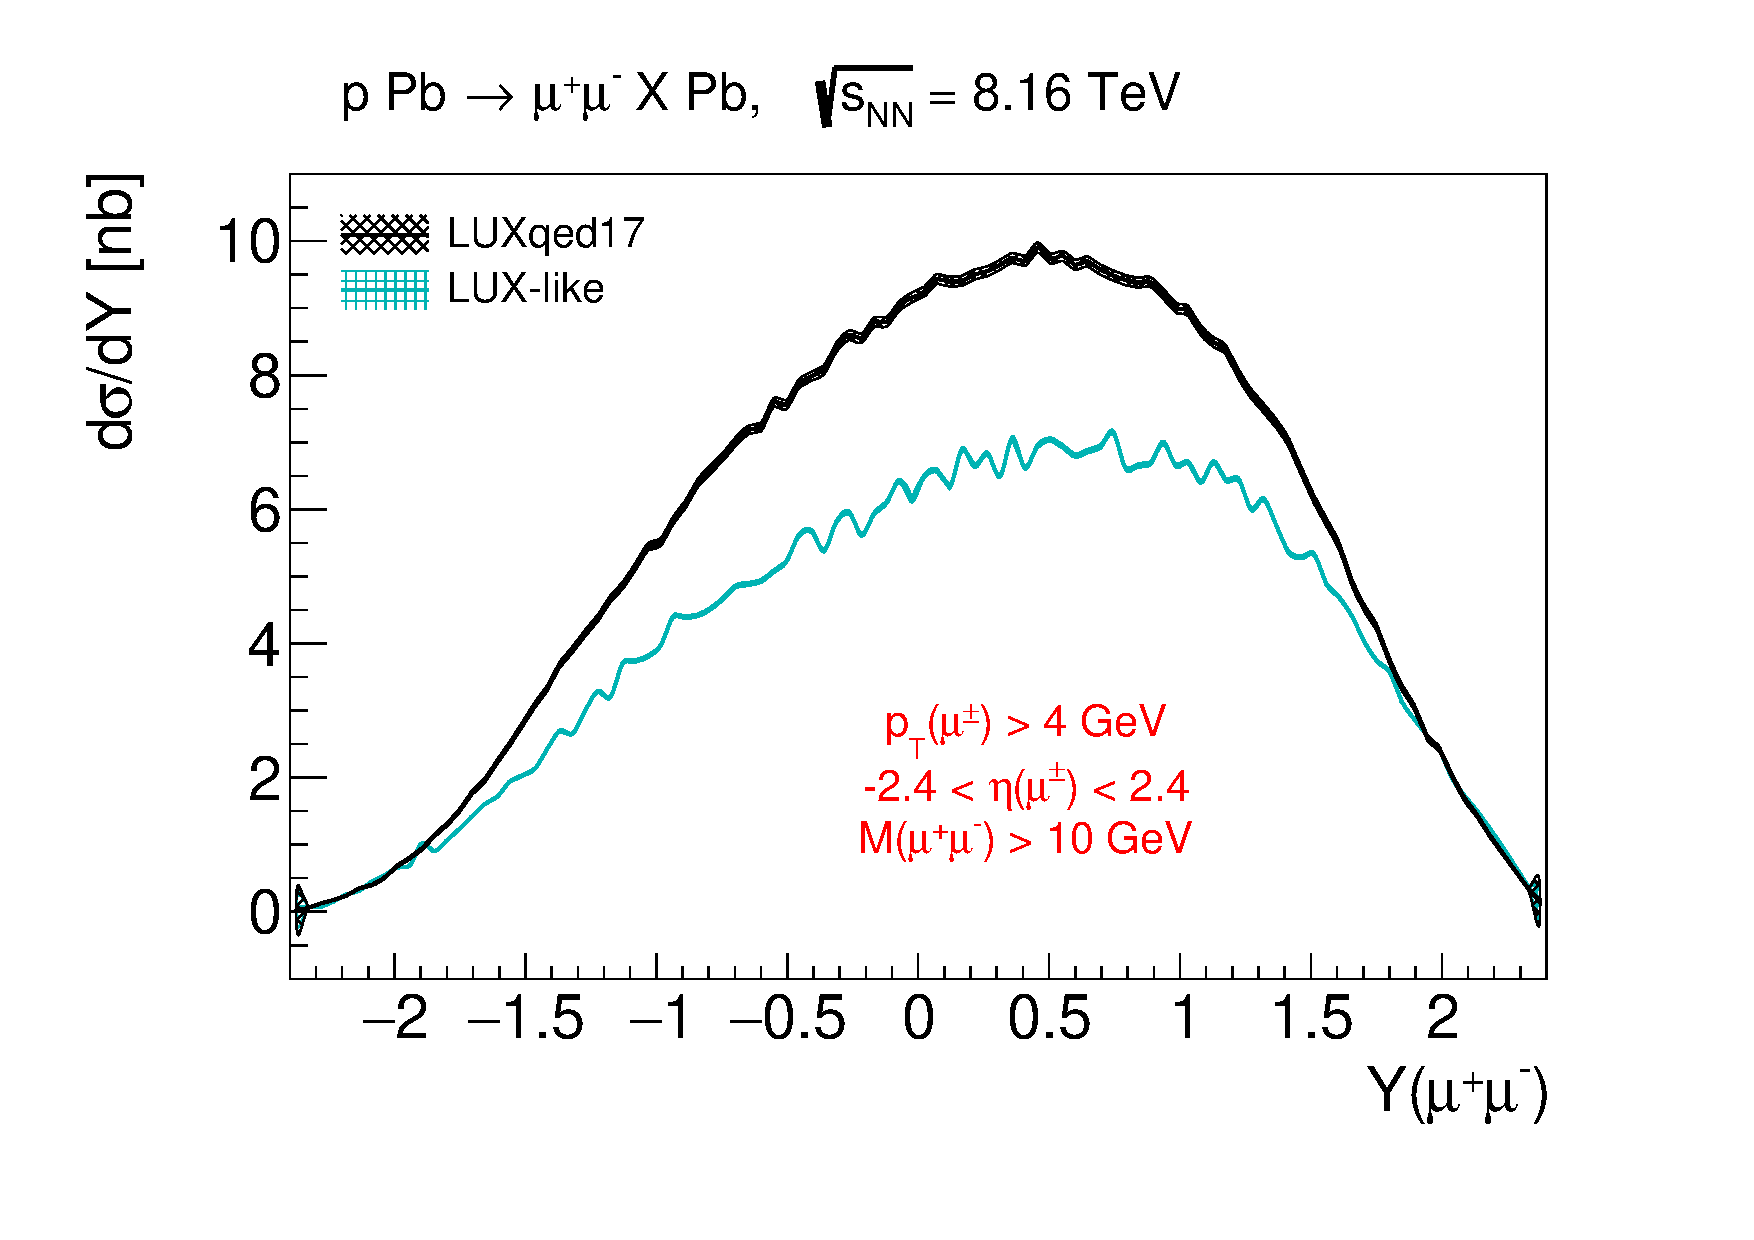
\includegraphics[width=0.43\textwidth]{figures/Yll_inc_cut_kt.pdf}
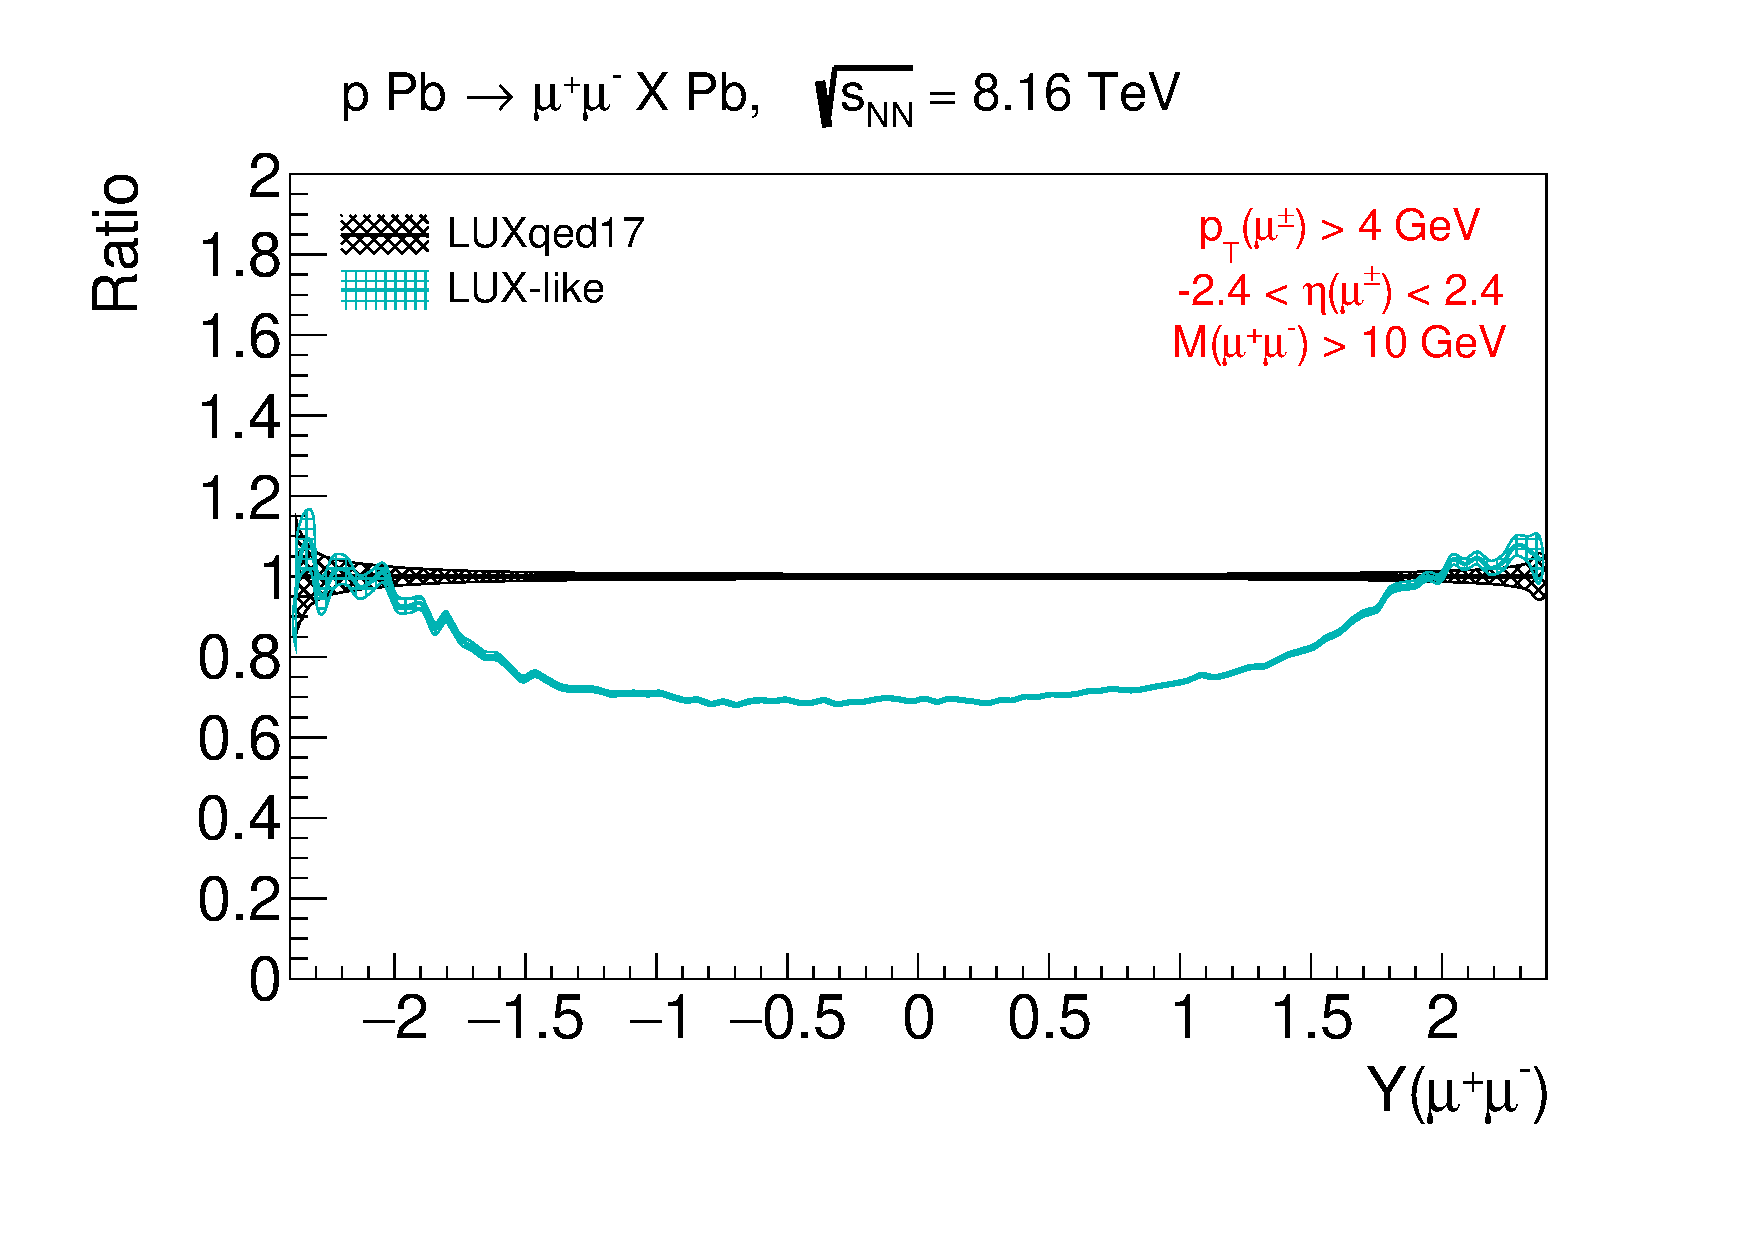
\includegraphics[width=0.43\textwidth]{figures/RatioYll_inc_cut_kt.pdf}
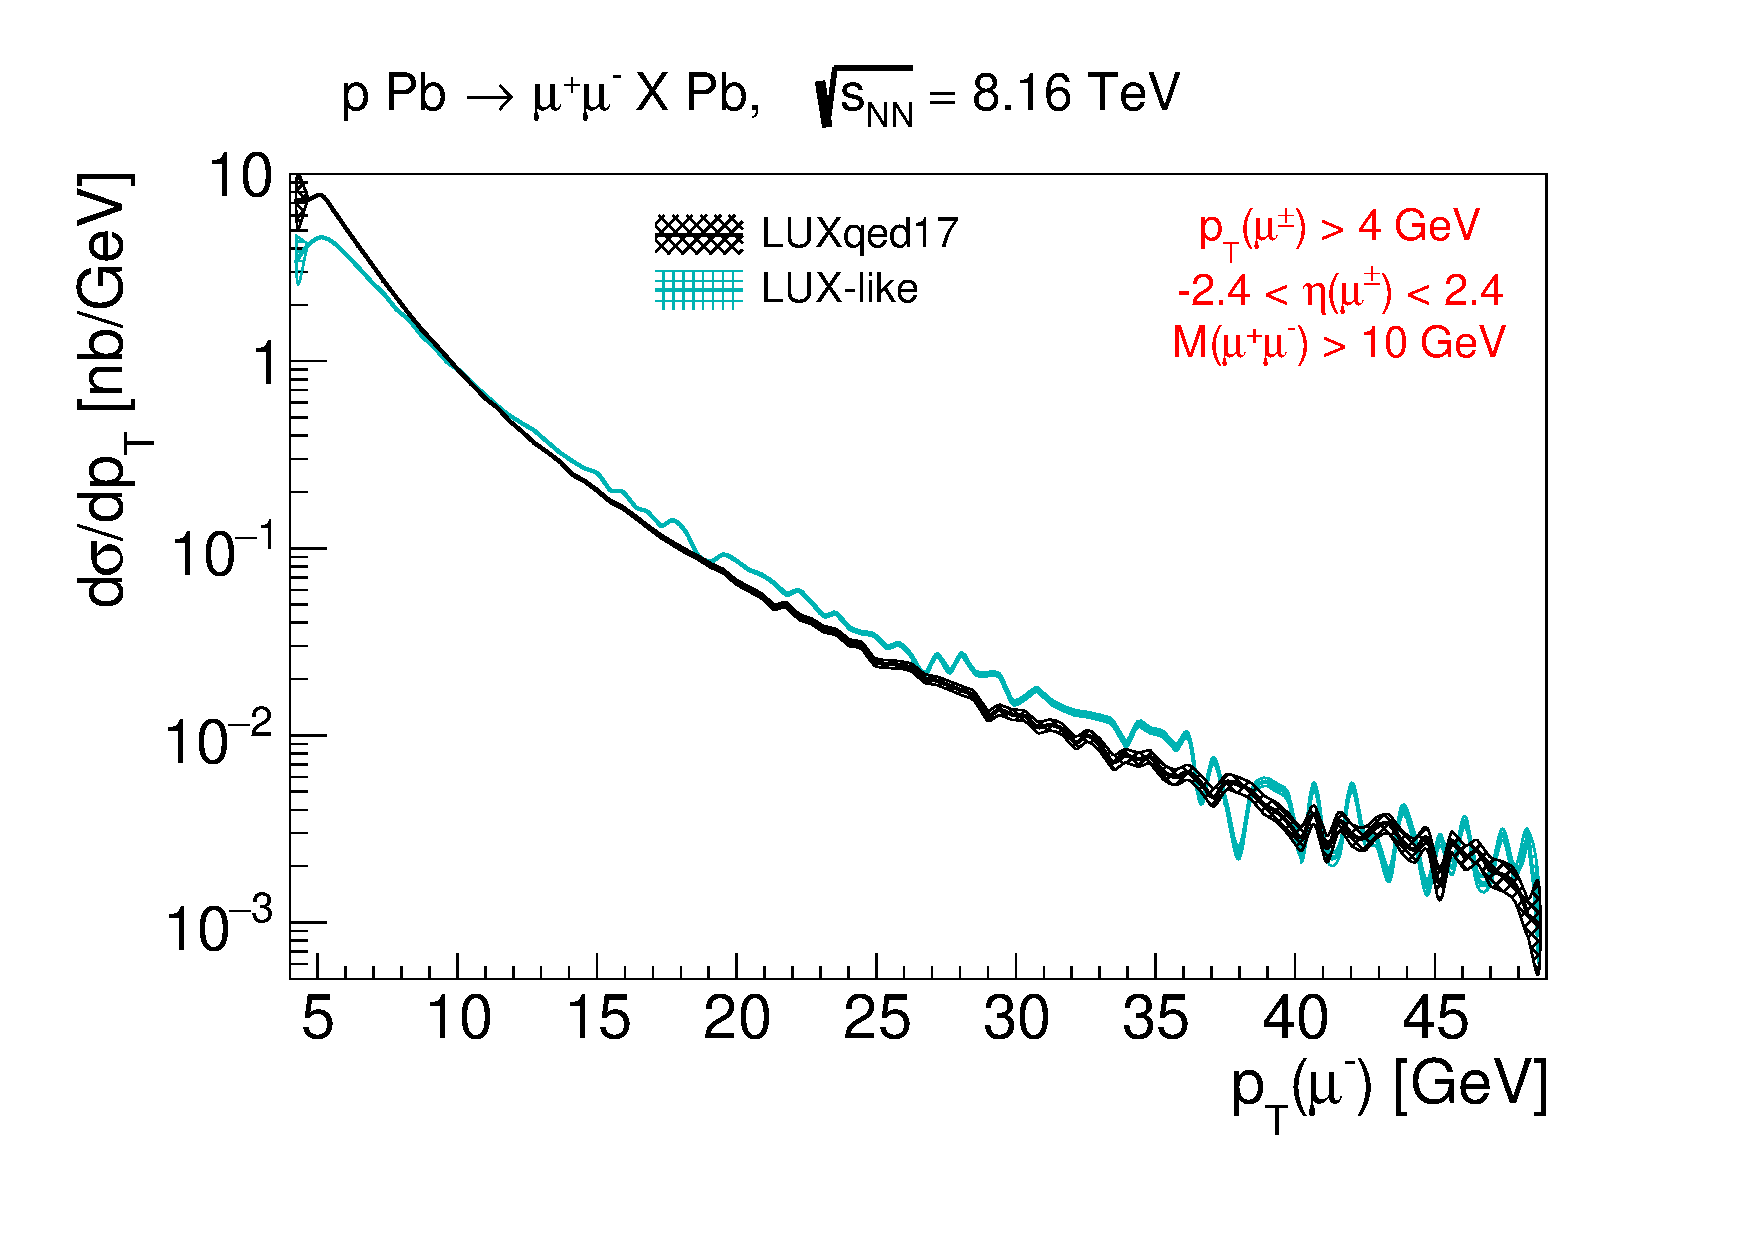
\includegraphics[width=0.43\textwidth]{figures/pTl_inc_cut_kt.pdf}
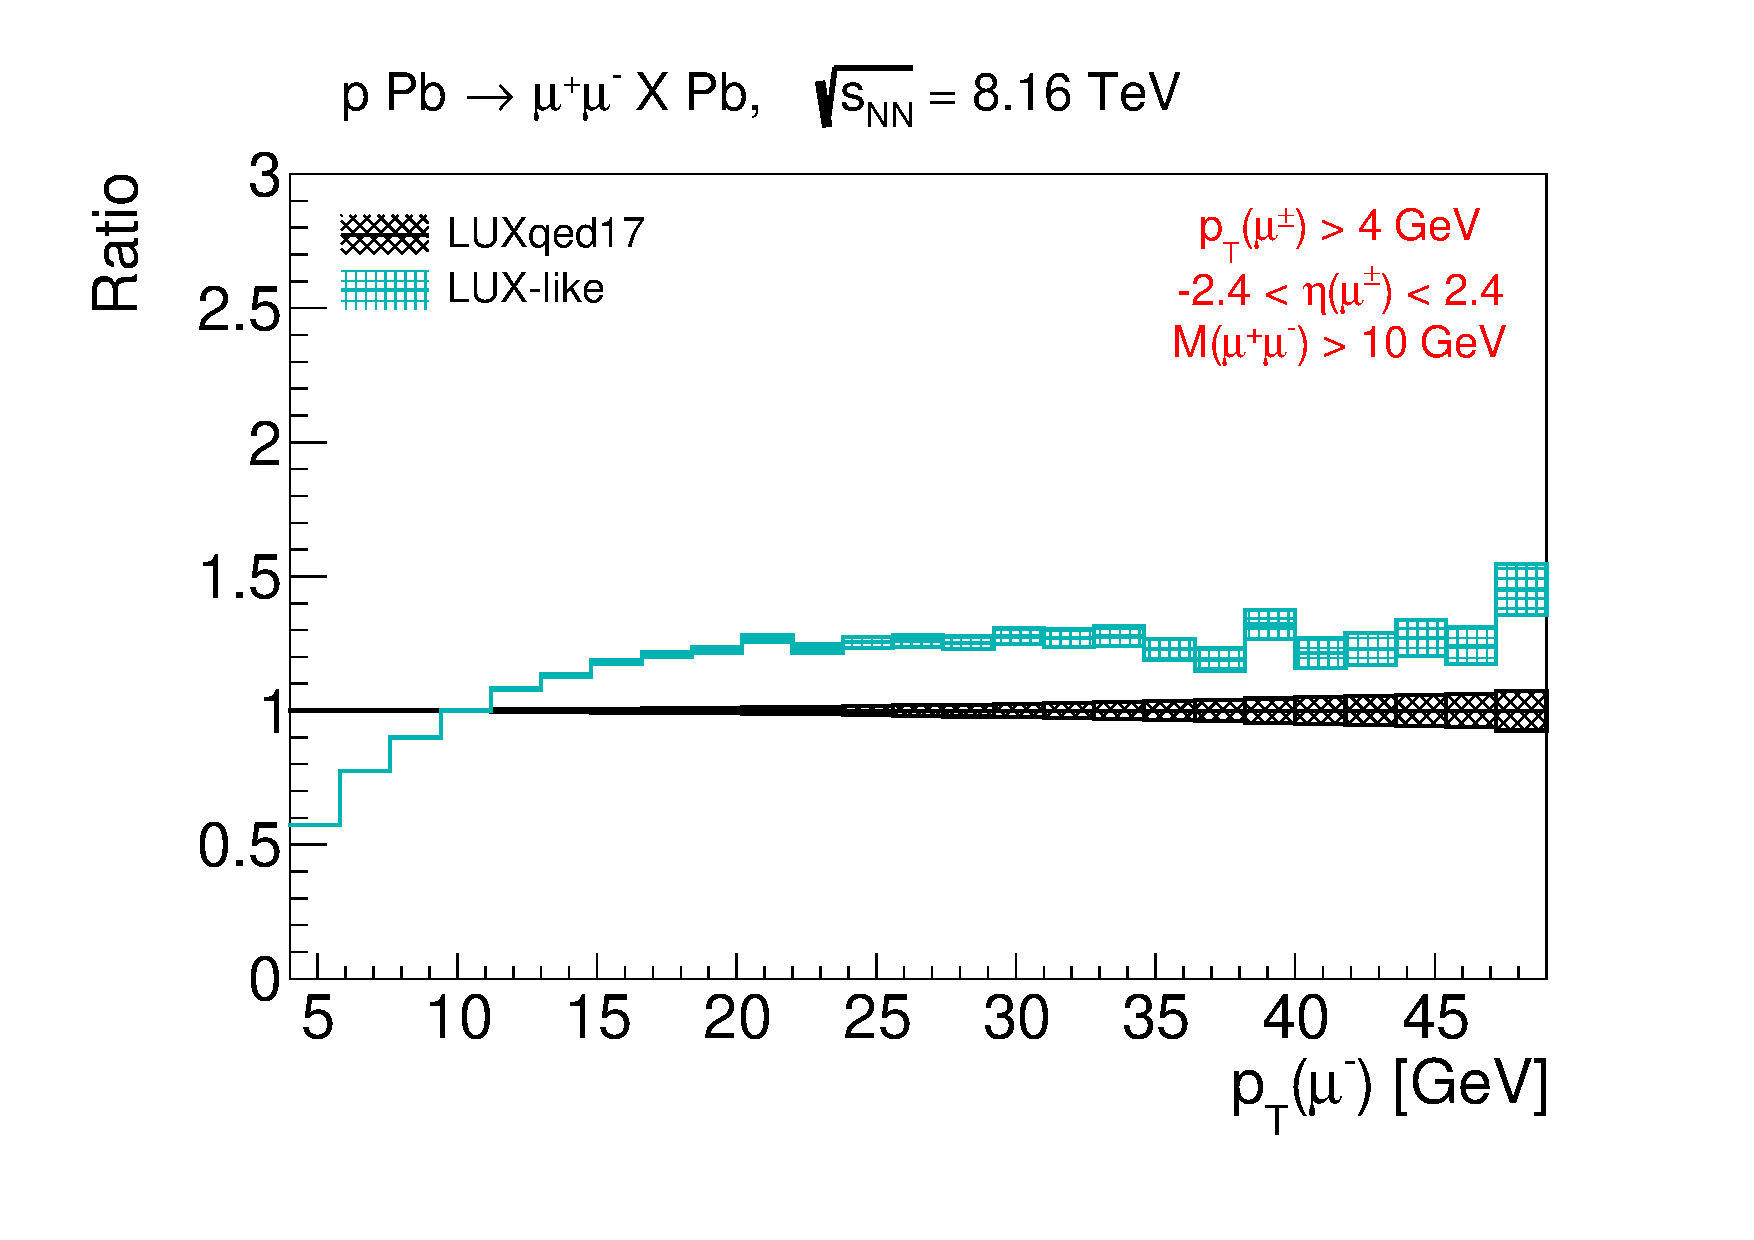
\includegraphics[width=0.43\textwidth]{figures/RatiopTl_inc_cut_kt.pdf}
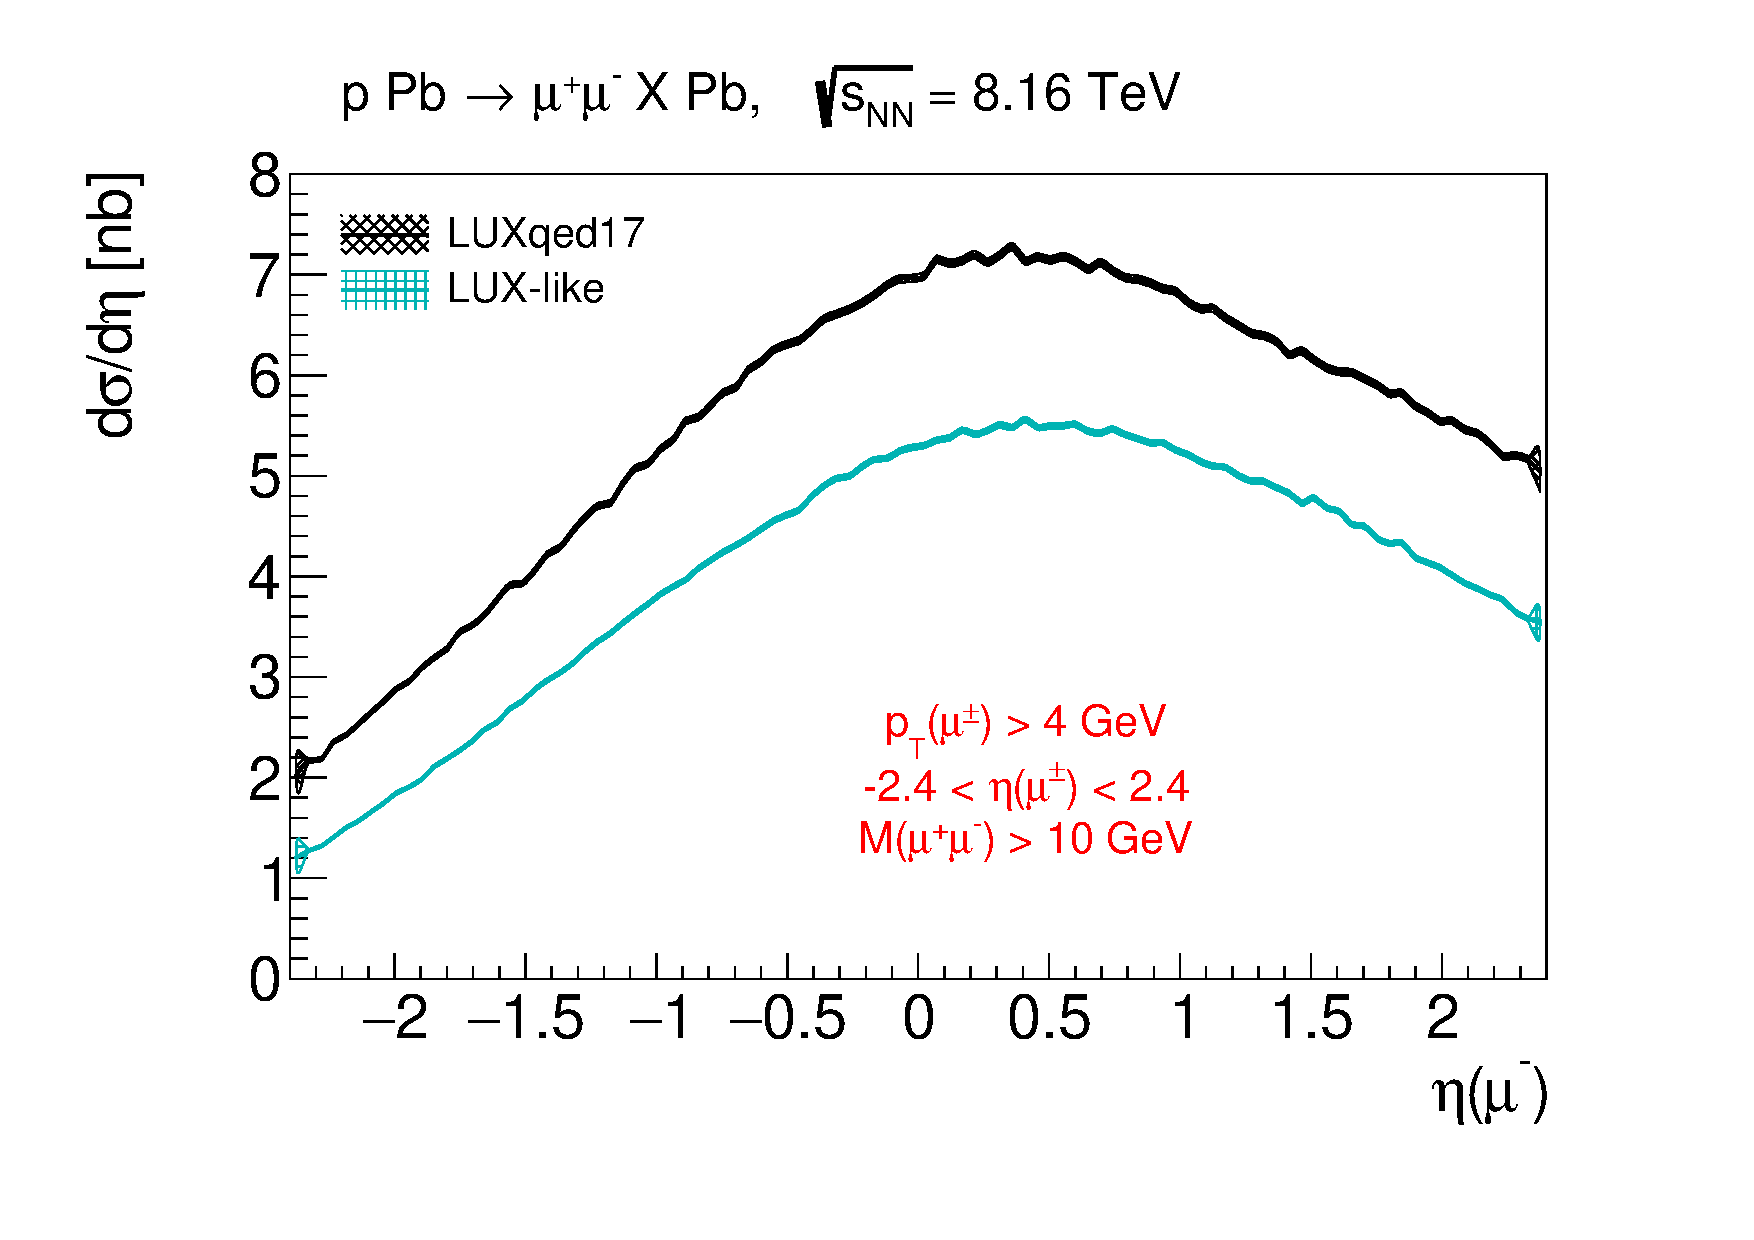
\includegraphics[width=0.43\textwidth]{figures/etal_inc_cut_kt.pdf}
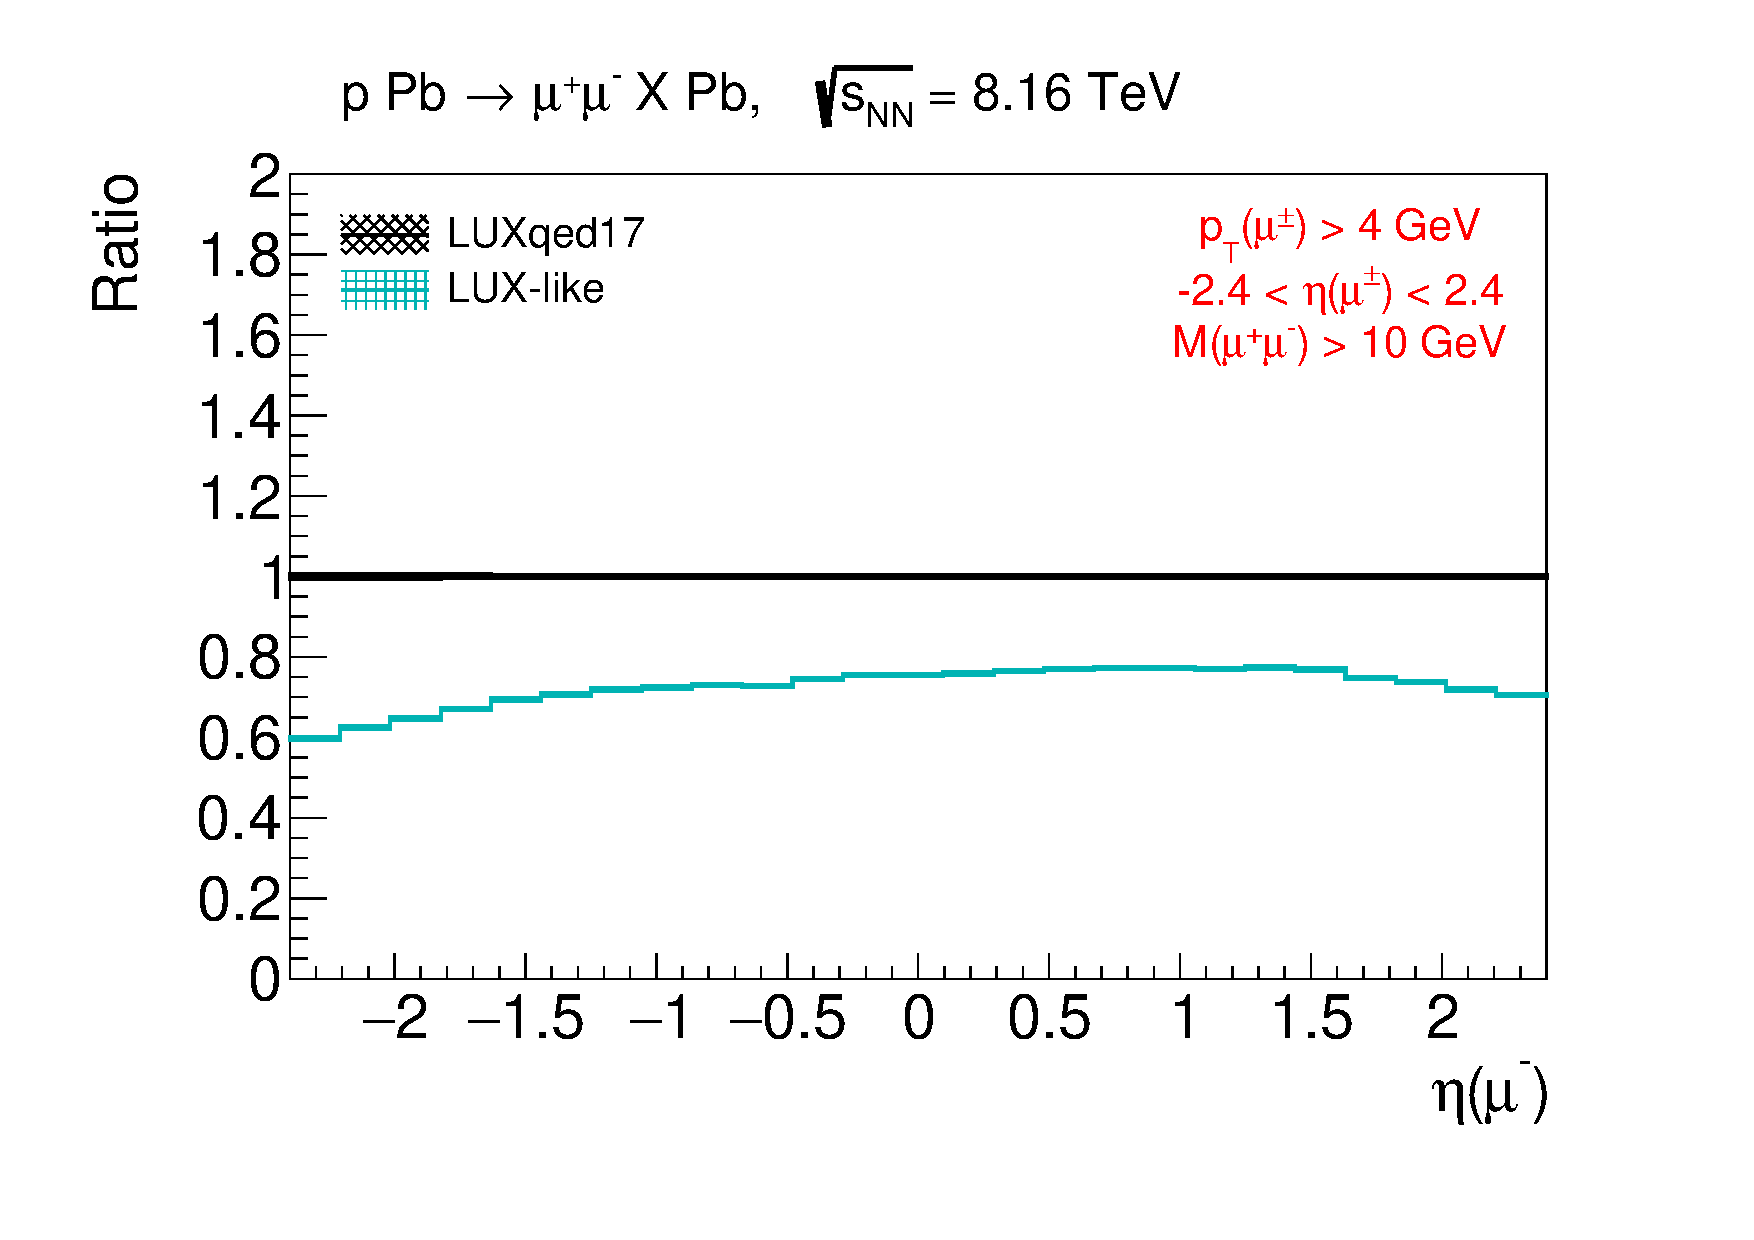
\includegraphics[width=0.43\textwidth]{figures/Ratioetal_inc_cut_kt.pdf}
\caption{Differential cross sections in the fiducial region for $p+\textrm{Pb}\rightarrow \textrm{Pb} + \ell^+\ell^- + X$ production at $\sqrt{s_{N N}} = 8.16$~\TeV\ for collinear LUXqed17 photon PDF and
for LUX-like $F_2+F_L$ photon PDF with $k_T$-factorization.
Four differential distributions are shown (from top to bottom): invariant mass of lepton pair, pair rapidity, transverse momentum of negatively-charged lepton and its pseudorapidity. Figures on the right show the ratios to LUXqed17 PDF.}
\label{fig:inc_cut_kt}
\end{figure}


\begin{table}[t]
\begin{center}
\begin{tabular}{|l|c|c|}
\hline
Contribution & Expected events ($C=1$) & Expected events ($C=0.7$) \\
\hline
%$\gamma^{p}_{\rm{el}}$ [$b_{min}=0.7fm$] & 45.5(2) nb & 17.3(1) nb\\
%\hline
$\gamma^{p}_{\rm{el}}$  & 3600 & 2500\\ % [Electric]
\hline
$\gamma^{p}_{\rm{inel}}$ [LUXqed17 collinear] & 5600 & 3900 \\
\hline
$\gamma^{p}_{\rm{inel}}$ [LUX-like $F_2+F_L$] & 3400 & 2400 \\
\hline
\end{tabular}
\end{center}
\caption{Expected number of events for $p+\textrm{Pb}\rightarrow \textrm{Pb} + \ell^+\ell^- + X$ production at $\sqrt{s_{N N}} = 8.16$~\TeV\ assuming $\int Ldt= 200~\textrm{nb}^{-1}$. 
Shown are several contributions: purely elastic, inelastic with collinear LUXqed17 PDF and inelastic with $k_T$-factorization and LUX-like $F_2+F_L$ proton structure function parameterization.
An effect of possible experimental efficiencies is shown in last column.}
\label{fig:numbers}
\end{table}

